\documentclass[a4paper,12pt]{article}
\usepackage{graphicx}
\usepackage{geometry}
\usepackage{fancyhdr}
\usepackage{hyperref}
\usepackage{array}

% Page layout settings
\setlength{\headheight}{14.5pt}
\geometry{top=1in, bottom=1in, left=1in, right=1in}

% Header and Footer settings
\pagestyle{fancy}
\fancyhf{}
\fancyhead[C]{Group 6}
\fancyfoot[C]{Page \thepage}

% Title page settings
\title{Lab Notebook}
\author{Group 6}
\date{\today}

\begin{document}

% Title Page
\begin{titlepage}
    \centering
    \vspace*{0.5in}
    
    {\Huge\bfseries Lab Notebook \\[0.2cm]}
    
\includegraphics[width=0.3\textwidth]{university_logo.png} \\[1.1cm]
    
    {\Large\bfseries Semester: 2 \\[0.5cm]}
    {\Large\bfseries Subject: Software Tools and Technology-I Lab \\[0.5cm]}
    {\Large\bfseries Group Number: 6 \\[0.5cm]}
    {\Large\bfseries Department: BCA and BSc \\[0.5cm]}
    
    {\Large \textbf{GitHub Repository:} \href{https://github.com/codeAtSin/group-6-final}{https://github.com/codeAtSin/group-6-final} \\[2cm]}
    
    \begin{tabular}{| l | c | c |}
        \hline
        \textbf{Name} & \textbf{Department} & \textbf{Roll Number} \\
        \hline
        Atul Sinha & BCA & 30001223022 \\
        \hline
        Neha Halder & BCA & 30001223046 \\
        \hline
        Arpan Singha Chowdhury & BCA & 30001223026 \\
        \hline
        Srija Saha & BSc & 30059223046 \\
        \hline
        Ankit Rai & BCA & 30001223060 \\
        \hline
    \end{tabular}

    \vfill

    {\large\bfseries MAKAUT \\ Information Technology}
\end{titlepage}

\newpage

% Table of Contents
\tableofcontents

\newpage

% Experiment/Assignment Section
\section{Assignment Details}
\textit{(Objective: To create a group lab book using \LaTeX \  and GitHub.)}
\begin{enumerate}
    \item Create a public Git repository.
    \item Add other members as collaborators.
    \item Push a LaTeX file in lab notebook format to the repository. The cover page should include:
    \begin{itemize}
        \item Each group member's name
        \item Roll number
        \item Department
    \end{itemize}
    \item Each member must write one lab notebook entry.
    \item Each member commits their entry to the Git repository.
\end{enumerate}

\newpage

% Individual Sections
{ \textbf{Date:} \today}
\section{Atul Sinha}

\subsection{Git Branching, Merging and Resolving conflicts}
In the given assignment I practiced git branching, merging and resolving the conflicts if any arrises.
\begin{enumerate}
    \item Created a new repository on GitHub named \texttt{git-advanced} then cloned it to my local machine.
    \item Created and switched to a new branch called \texttt{feature-1}.
    \item I created a file named \texttt{shared.txt} with the following content:
    \begin{verbatim}
    This is a shared file.
    Line 1: Original text.
    Line 2: Original text.
    \end{verbatim}
    \item Then staged and committed the file with a meaningful message to push it to GitHub.
    \item Created and switched to another branch called \texttt{feature-2}.
    \item Checked out the \texttt{shared.txt} file from the main branch, modified \texttt{shared.txt} to include.
    \begin{verbatim}
    Line 2: Modified text in feature-2.
    \end{verbatim}
    \item Staged and committed the changes with a meaningful message and pushed to GitHub.
    \item Switched back to the \texttt{feature-1} branch and modified \texttt{shared.txt} to include:.
    \begin{verbatim}
    Line 2: Modified text in feature-1.
    \end{verbatim}
    \item Staged and committed the changes with a meaningful message and then pushed to GitHub.
    \item Merged \texttt{feature-1} into the main branch.
    \item Merged \texttt{feature-2} into the main branch, which introduced a conflict.
    \item Then resolved the conflict by editing the file and committed the resolution.
    \item Finally pushed the updated main branch to GitHub.
    \item Then deleted the \texttt{feature-1} and \texttt{feature-2} branches.
\end{enumerate}
\href{https://github.com/codeAtSin/git-advanced}{CLICK: GitHub Repo for this assignment}
\par\vspace{2em}
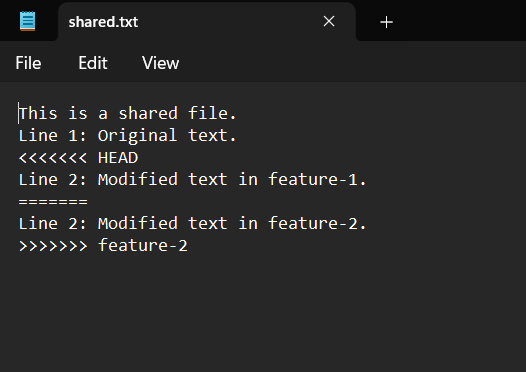
\includegraphics[width=0.8\textwidth]{conflictfile.png}
\par\vspace{2em}
\large\textbf{Showing conflicts in file.}
\par\vspace{2em}
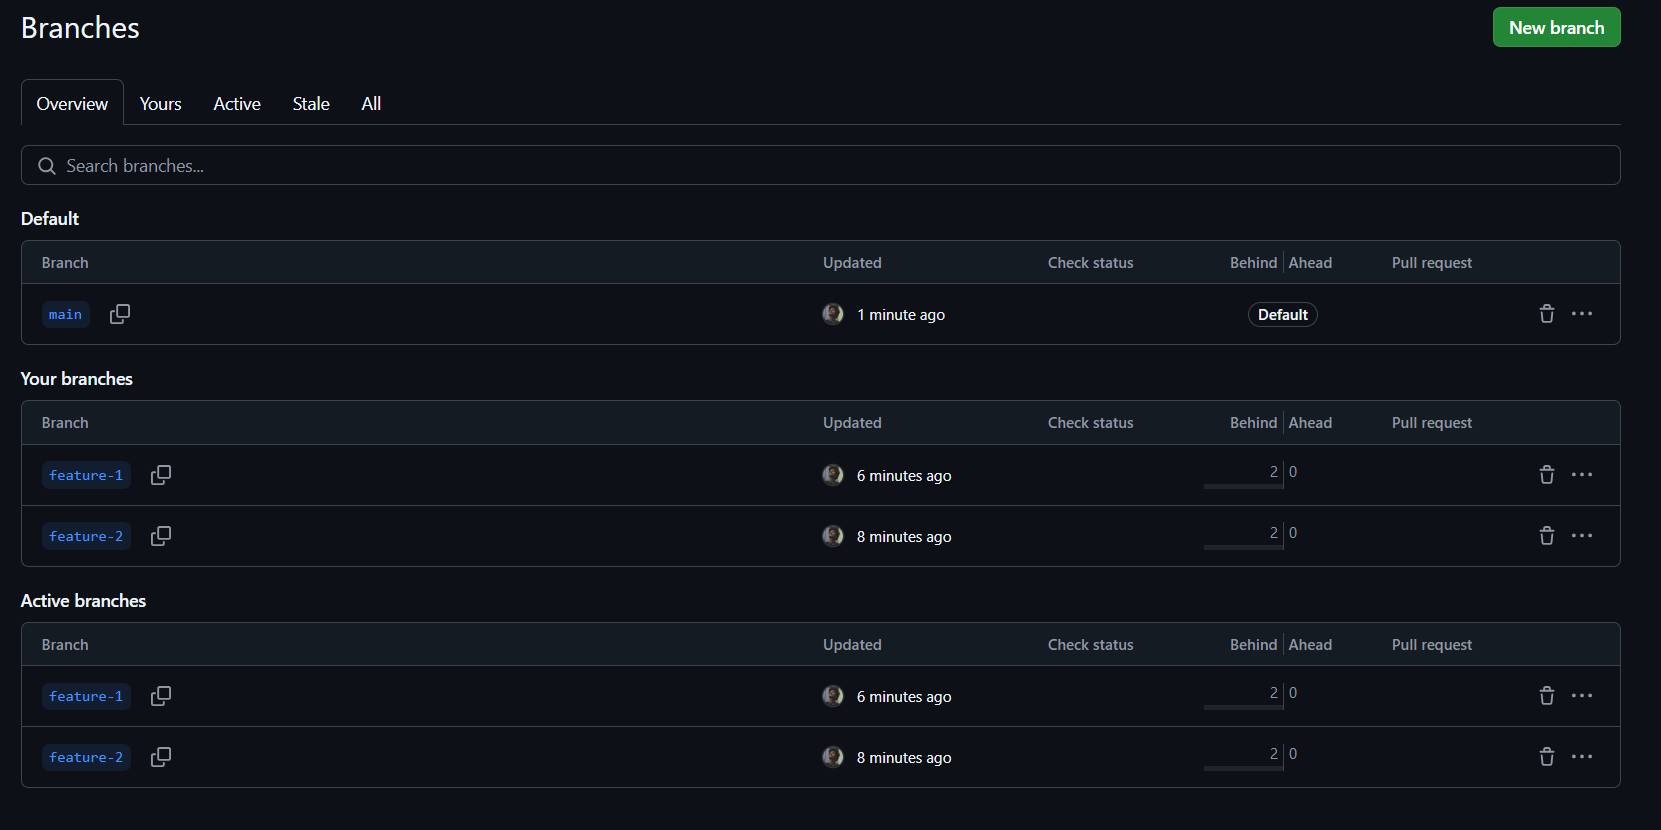
\includegraphics[width=0.7\textwidth]{allpushes.png}
\par\vspace{2em}
\large\textbf{Screenshots showing all the pushes in the repo.}
\vspace{0.3in}

\newpage
\end{document}